\documentclass[tikz,border=2pt]{standalone}
\usepackage{tikz}
\usetikzlibrary{positioning}
\begin{document}
% Namikawa--Ueno type: IV^*-III^*-t
% Target MRNC type: IV^*-III^*-t
% Adapted from Tim Dokchitser picture: IV^*\e({\it n})III^*
% Parameter substitution: n -> t
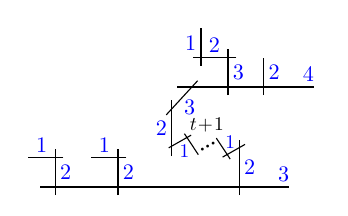
\begin{tikzpicture}[xscale=0.57,yscale=0.62]
\draw[thick,shorten >=2] (4/15,0)--(89/15,0) node[inner sep=2pt,blue,above left,scale=0.8] {3};
\draw[shorten <=-3pt, shorten >=-3pt] (3/5,0)--node[inner sep=2pt,scale=0.8,blue,right] {2} (3/5,3/5);
\draw[shorten <=-3pt] (3/5,3/5)--node[inner sep=2pt,scale=0.8,blue,above] {1} (0,3/5);
\draw[shorten <=-3pt, shorten >=-3pt] (2,0)--node[inner sep=2pt,scale=0.8,blue,right] {2} (2,3/5);
\draw[shorten <=-3pt] (2,3/5)--node[inner sep=2pt,scale=0.8,blue,above] {1} (7/5,3/5);
\draw[shorten <=-3pt, shorten >=-3pt] (47/10,0)--node[inner sep=2pt,scale=0.8,blue,right] {2} (47/10,4/5);
\draw (47/10,4/5) 
    ++(0.13,0.07)--++(-0.5,-0.26)++(0.19,0.12)  
    ++(-0.02,0)
      node[blue,scale=0.7,inner sep=1,anchor=south]{1}
    ++(0.02,0)
    ++(-0.02,-0.16)--++(-0.31,0.43)++(-0.07,-0.13)  
    node{$\cdot$} ++(-0.12,-0.06) node{$\cdot$}
    ++(-0.12,-0.06) node{$\cdot$}++(0.1,0.17)    node[auto,inner sep=5,scale=0.7,anchor=south]{$t\!+\!1$}
    ++(-0.19,-0.26)--++(-0.31,0.43)++(-0.04,-0.18)   
    ++(0.04,0)
      node[blue,scale=0.7,inner sep=1,anchor=north]{1}
    ++(-0.04,0)
    ++(0.04,0.18)++(0.15,-0.03)--++(-0.5,-0.26);
\draw[shorten <=-3pt, shorten >=-3pt] (16/5,4/5)--node[inner sep=2pt,scale=0.8,blue,left] {2} (16/5,8/5);
\draw[shorten <=-3pt, shorten >=-3pt] (16/5,8/5)--node[inner sep=2pt,scale=0.8,blue,below right=-1pt and -1pt] {3} (73/20,41/20);
\draw[thick,shorten >=2] (199/60,41/20)--(389/60,41/20) node[inner sep=2pt,blue,above left,scale=0.8] {4};
\draw[shorten <=-3pt, shorten >=-3pt] (89/20,41/20)--node[inner sep=2pt,scale=0.8,blue,right] {3} (89/20,53/20);
\draw[shorten <=-3pt, shorten >=-3pt] (89/20,53/20)--node[inner sep=2pt,scale=0.8,blue,above] {2} (77/20,53/20);
\draw[shorten <=-3pt] (77/20,53/20)--node[inner sep=2pt,scale=0.8,blue,left] {1} (77/20,13/4);
\draw[shorten <=-3pt] (21/4,41/20)--node[inner sep=2pt,scale=0.8,blue,right] {2} (21/4,53/20);
\end{tikzpicture}
\end{document}
